\documentclass[11pt]{article}
\usepackage{amsmath}
\title{\textbf{Theory of Computation}}
\author{Homework 2\\
					\\
		Qing-Cheng Li\\
		R01922024}
\date{\today}
\usepackage{graphicx}
\begin{document}

\maketitle
\section{Problem 1}
\subsection{CNF}
\begin{align*}
 \phi &\equiv ((a \wedge \neg b ) \vee (\neg c \wedge d)) \Rightarrow (e \Rightarrow \neg f) \\
 &\equiv ((a \wedge \neg b ) \vee (\neg c \wedge d)) \Rightarrow \neg (e \wedge f) \\
 &\equiv \neg (((a \wedge \neg b ) \vee (\neg c \wedge d)) \wedge (e \wedge f)) \\
 &\equiv (\neg a \vee b \vee \neg e \vee \neg f) \wedge (c \vee \neg d \vee \neg e \vee \neg f)
\end{align*}

\subsection{Boolean Circuit}
\begin{figure}[htp]
\centering
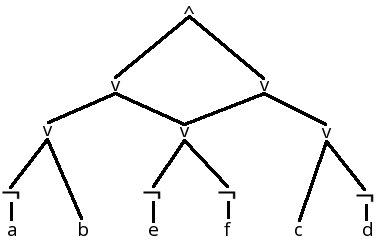
\includegraphics[scale=0.3]{hw2_boolean_circuit.png}
\label{}
\end{figure}

\section{Problem 2}
Given question ``$M;x \in H$", we can construct a machine $M'(y)$: \textbf{If} $y = x$ \textbf{then} $M(x)$ \textbf{else} ``no". If $y = x$, run $M$ on x, if $M$ halts on state ``yes", $M'$ accepts $y$, if $M$ halts on ``no", $M'$ rejects $y$. If $y \neq x$, $M'$ rejects $y$. So $M'$ is a TM that accepts some input. We know that $H$ is undecidable, so $L$ is undecidable. 



\end{document}
